 

\documentclass[12pt]{article}
\usepackage{times}
\usepackage{indentfirst}
\usepackage{graphicx}
\usepackage{multirow}
\usepackage{float}
\usepackage{amsmath}
\graphicspath{ {./img/} }
%Setup the layout of the pages
\topmargin 0.0cm
\oddsidemargin 0.2cm
\textwidth 16cm 
\textheight 21cm
\footskip 1.0cm


\title{
    Machine Learning Review\\
}
\author{Molin Liu}

\begin{document}

\maketitle

\section*{Introduction}

This is a review work for the Machine Learning course in
\textit{Univeristy of Glasgow}.

\section{Regression}

\subsection{Linear Regression}

For $x = (x_1, x_2, ..., x_m)$, 
where $x_i$ is the $i_{th}$ attribute of $x$, 
a lenear model tries to train a linear combination function
from these attributes, i.e:
$$f(x) = w_1 x_1 + w_2 x_2 +...+ w_m x_m+b$$
which can be written in vector as:
$$f(x)=w^Tx+b$$
where $w=(w_1, w_2,...,w_m)$.

The linear regression model is trained by \textit{loss function}.
Generally, we define our \textit{loss function} as:
$$min\sum_{i=1}^{m}{(y_i-f(x_i))^2}$$

\subsubsection{Loss Function}

There are several kinds of \textit{loss functions} we can choose from.

- \textbf{L1-norm}: L1-norm can be represented as follow:
$$S=\sum_{i=1}^{m}\left|y_{i}-f\left(x_{i}\right)\right|$$

- \textbf{L2-norm}: L2-norm is what we used above:
$$S=\sum_{i=1}^{m}\left(y_{i}-f\left(x_{i}\right)\right)^{2}$$

\subsubsection{Least Square Solution}
The solution of \textbf{Least Square} is:
$$
\vec{w}=\left(X^{\top} X\right)^{-1} X^{\top} Y
$$

\textbf{Prove:}

The error vector $(Y-X \vec{w})$ should be orthogonal to every column of $X$:
$$
(Y-X \vec{w}) \cdot X_{j}=0
$$

which can be written as a matrix equation:
$$
(Y-X \vec{w})^{\top} X=\overrightarrow{0}
$$

Then we can easily derive the equation from the following process:
$$
\begin{aligned} X^{\top}(Y-X \vec{w}) &=X^{\top} Y-X^{\top} X \vec{w}=0 \\ \Longrightarrow &\left(X^{\top} X\right) \vec{w}=X^{\top} Y \\ \Longrightarrow \quad \vec{w}=\left(X^{\top} X\right)^{-1} X^{\top} Y \end{aligned}
$$
\subsubsection{Conclusion}

\subsection{Polynomial Regression}

The \textbf{Polynomial Regression} can be written as:
$$
t=w_{0}+w_{1} x+w_{2} x^{2}+w_{3} x^{2}+\ldots+w_{K} x^{K}=\sum_{k=0}^{\kappa} w_{k} x^{k}
$$

Define the loss funcion:
$$
\mathcal{L}=\frac{1}{N}(\mathbf{t}-\mathbf{X} \mathbf{w})^{\top}(\mathbf{t}-\mathbf{X} \mathbf{w})
$$
\subsubsection{Generalization \& Overfitting}

We can find out that the \textbf{loss} will always decrease
as the model is made more complex.

How to choose the right model complexity?
\textbf{Cross-validation}

\subsubsection{Cross-Validation}

\section{Classification}

The \textbf{Classification} task is to classify
a set of \textit{N} objects $x_i$ with attributes.
Each object has an associated label $t_i$

\textbf{Probabilistic classifier} produce a probability of class membership:

$P(t_{\text {new}}=k | \mathbf{x}_{\text {new }}, \mathbf{X}, \mathbf{t})$

\textbf{non-Probabilistic classifier} produce a hard assignment:

$t_{new}=1$ or $t_{new}=0$

\subsection{KNN}

K-Nearest Neighbours(KNN)

- Non-probabilistic classifier;

- Supervised trainning;

- Fast;

- We can use CV to find the right $K$;

\subsubsection{Problem}
- As $K$ increases, the small classes will disppear.

\subsection{Logistic Regression}

\subsection{SVM}
\subsubsection{Hard Margin}
If the training data is linearly seperable,
we can select two parallel hyperplanes that separate the two classes of data,
so that the distance between them is as large as possible.

These hyperplanes can be described by the equations:
$$
\vec{w} \cdot \vec{x}_{i}-b \geq 1, \text { if } y_{i}=1
$$
or
$$
\vec{w} \cdot \vec{x}_{i}-b \leq-1, \text { if } y_{i}=-1
$$

We can easily infer that 
$$
y_{i}\left(\vec{w} \cdot \vec{x}_{i}-b\right) \geq 1, \quad \text { for all } 1 \leq i \leq n
$$

We want to maximise $\gamma=\frac{1}{\|\mathbf{w}\|}$,
equivalent to minimising $\|\mathbf{w}\|$

Note: $y_i$ is the label in the data, which is in $\{-1, 1\}$,
rather than vertical axis value of the data.
\begin{figure}[H]
    \center
    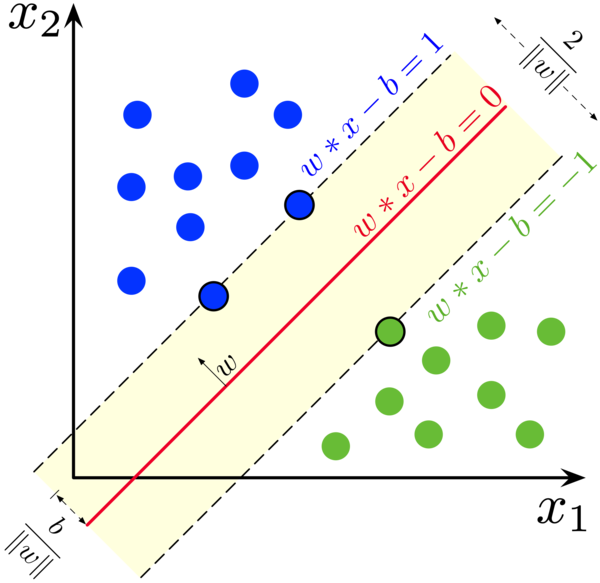
\includegraphics{img/600px-SVM_margin.png}
    \caption{Hard margin}
    \label{fig:svm_hard_margin}
\end{figure}

\subsubsection{Soft Margin}
Soft-margin function for the data are not linearly seperable.

\subsubsection{Inner Product}

\section{ROC}
Sensitivity/Recall

$$
S_{e}=\frac{T P}{T P+F N}
$$

Specificity

$$
S_{p}=\frac{T N}{T N+F P}
$$

\section{Unsupervised Learning}
\subsection{K-Means}

\subsection{Gaussion Mixture Model}
\end{document}

